\chapter{Конструкторская часть}

\section{Описание сущностей проектируемой базы данных}

База данных содержит 13 таблиц:

\begin{enumerate}
	\item Таблица \guillemotleft Coach\guillemotright хранит информацию о тренерах. Содержит следующие поля:
	\begin{itemize}[label=—]
		\item ID -- первичный ключ;
		\item name -- имя;
		\item surname -- фамилия;
		\item login -- логин;
		\item password -- пароль в защищённом виде;
		\item is\_participate -- статус тренера(уволен, работает).
	\end{itemize}
	\item Таблица \guillemotleft CoachSchedule\guillemetright хранит информацию о рабочих часах тренера. Содержит следующие поля:
	\begin{itemize}[label=—]
		\item ID -- первичный ключ;
		\item CoachID -- идентификатор тренера;
		\item date -- дата в формате ГГГГ-ММ-ДД;
		\item start -- время начала работы в формате ЧЧ:ММ:СС;
		\item stop -- время окончания работы в формате ЧЧ:ММ:СС.
	\end{itemize}
	\item Таблица \guillemotleft Hall\guillemetright хранит информацию о спортивных пространствах. Содержит следующие поля:
	\begin{itemize}[label=—]
		\item ID -- первичный ключ;
		\item name -- название.
	\end{itemize}
	\item Таблица \guillemotleft CoachSpecializationTypes\guillemetright хранит информацию о видах тренерских специализаций. Содержит следующие поля:
	\begin{itemize}[label=—]
		\item ID -- первичный ключ;
		\item name -- название;
		\item HallID -- идентификатор спортивного пространства для проведения тренировок тренером с такой специализацией.
	\end{itemize}
	\item Таблица \guillemotleft CoachSpecialization\guillemetright хранит информацию о тренерах и какие специализации у них есть. Содержит следующие поля:
	\begin{itemize}[label=—]
		\item ID -- первичный ключ;
		\item SpecID -- идентификатор типа специализации;
		\item CoachID -- идентификатор тренера.
	\end{itemize}
	\item Таблица \guillemotleft HallSchedule\guillemetright хранит информацию о расписании работы спортивных пространств. Содержит следующие поля:
	\begin{itemize}[label=—]
		\item ID -- первичный ключ;
		\item HallID -- идентификатор спортивного пространства;
		\item date -- дата в формате ГГГГ-ММ-ДД;
		\item start -- время начала работы в формате ЧЧ:ММ:СС;
		\item stop -- время окончания работы в формате ЧЧ:ММ:СС.
	\end{itemize}
	\item Таблица \guillemotleft Admin\guillemotright хранит информацию об администраторах. Содержит следующие поля:
	\begin{itemize}[label=—]
		\item ID -- первичный ключ;
		\item name -- имя;
		\item surname -- фамилия;
		\item login -- логин;
		\item password -- пароль в защищённом виде;
		\item is\_participate -- статус администратора(уволен, работает).
	\end{itemize}
	\item Таблица \guillemotleft StandartTraining\guillemotright хранит информацию о групповых тренировках и мероприятиях. Содержит следующие поля:
	\begin{itemize}[label=—]
		\item ID -- первичный ключ;
		\item name -- название;
		\item AdminID -- идентификатор администратора, создавшего мероприятие;
		\item CoachID -- идентификатор тренера;
		\item HallID -- идентификатор спортивного пространства;
		\item capacity -- количество мест на мероприятие;
		\item datetime -- дата и время начала мероприятия в формате ГГГГ-ММ-ДД ЧЧ:ММ:СС;
		\item duration -- продолжительность.
	\end{itemize}
	\item Таблица \guillemotleft Client\guillemotright хранит информацию о клиентах. Содержит следующие поля:
	\begin{itemize}[label=—]
		\item ID -- первичный ключ;
		\item name -- имя;
		\item surname -- фамилия;
		\item login -- логин;
		\item password -- пароль в защищённом виде;
		\item is\_participate -- статус клиента(ходит, перестал ходить).
	\end{itemize}
	\item Таблица \guillemotleft ClientDynamicTypes\guillemotright хранит информацию о возможных видах персональных клиентских статистик для отслеживания. Содержит следующие поля:
	\begin{itemize}[label=—]
		\item ID -- первичный ключ;
		\item name -- название статистики;
		\item unit -- мера измерения.
	\end{itemize}
	\item Таблица \guillemotleft ClientDynamic\guillemotright хранит информацию о клиентах и их персональных статистиках. Содержит следующие поля:
	\begin{itemize}[label=—]
		\item ID -- первичный ключ;
		\item ClientID -- идентификатор клиента;
		\item DynamicTypeID -- идентификатор типа статистики;
		\item value -- зафиксированное значение;
		\item date -- дата измерения в формате ГГГГ-ММ-ДД.
	\end{itemize}
	\item Таблица \guillemotleft TrainingSigns\guillemotright хранит информацию о клиентах и их записях на групповые мероприятия и тренировки. Содержит следующие поля:
	\begin{itemize}[label=—]
		\item ID -- первичный ключ;
		\item ClientID -- идентификатор клиента;
		\item StdTrainingID -- идентификатор группового мероприятия.
	\end{itemize}
	\item Таблица \guillemotleft IndividualTraining\guillemotright хранит информацию об индивидуальных тренировках. Содержит следующие поля:
	\begin{itemize}[label=—]
		\item ID -- первичный ключ;
		\item CoachID -- идентификатор тренера;
		\item ClientID -- идентификатор клиента;
		\item HallID -- идентификатор спортивного пространства;
		\item datetime -- дата и время начала тренировки в формате ГГГГ-ММ-ДД ЧЧ:ММ:СС;
		\item duration -- продолжительность;
		\item notes -- некоторые дополнительные заметки о тренировке.
	\end{itemize}
\end{enumerate}

\section{Диаграмма проектируемой базы данных}

На рисунке \ref{fig:database_diagram} представлена диаграмма проектируемой
базы данных.

\begin{figure}[H]
	\centering
	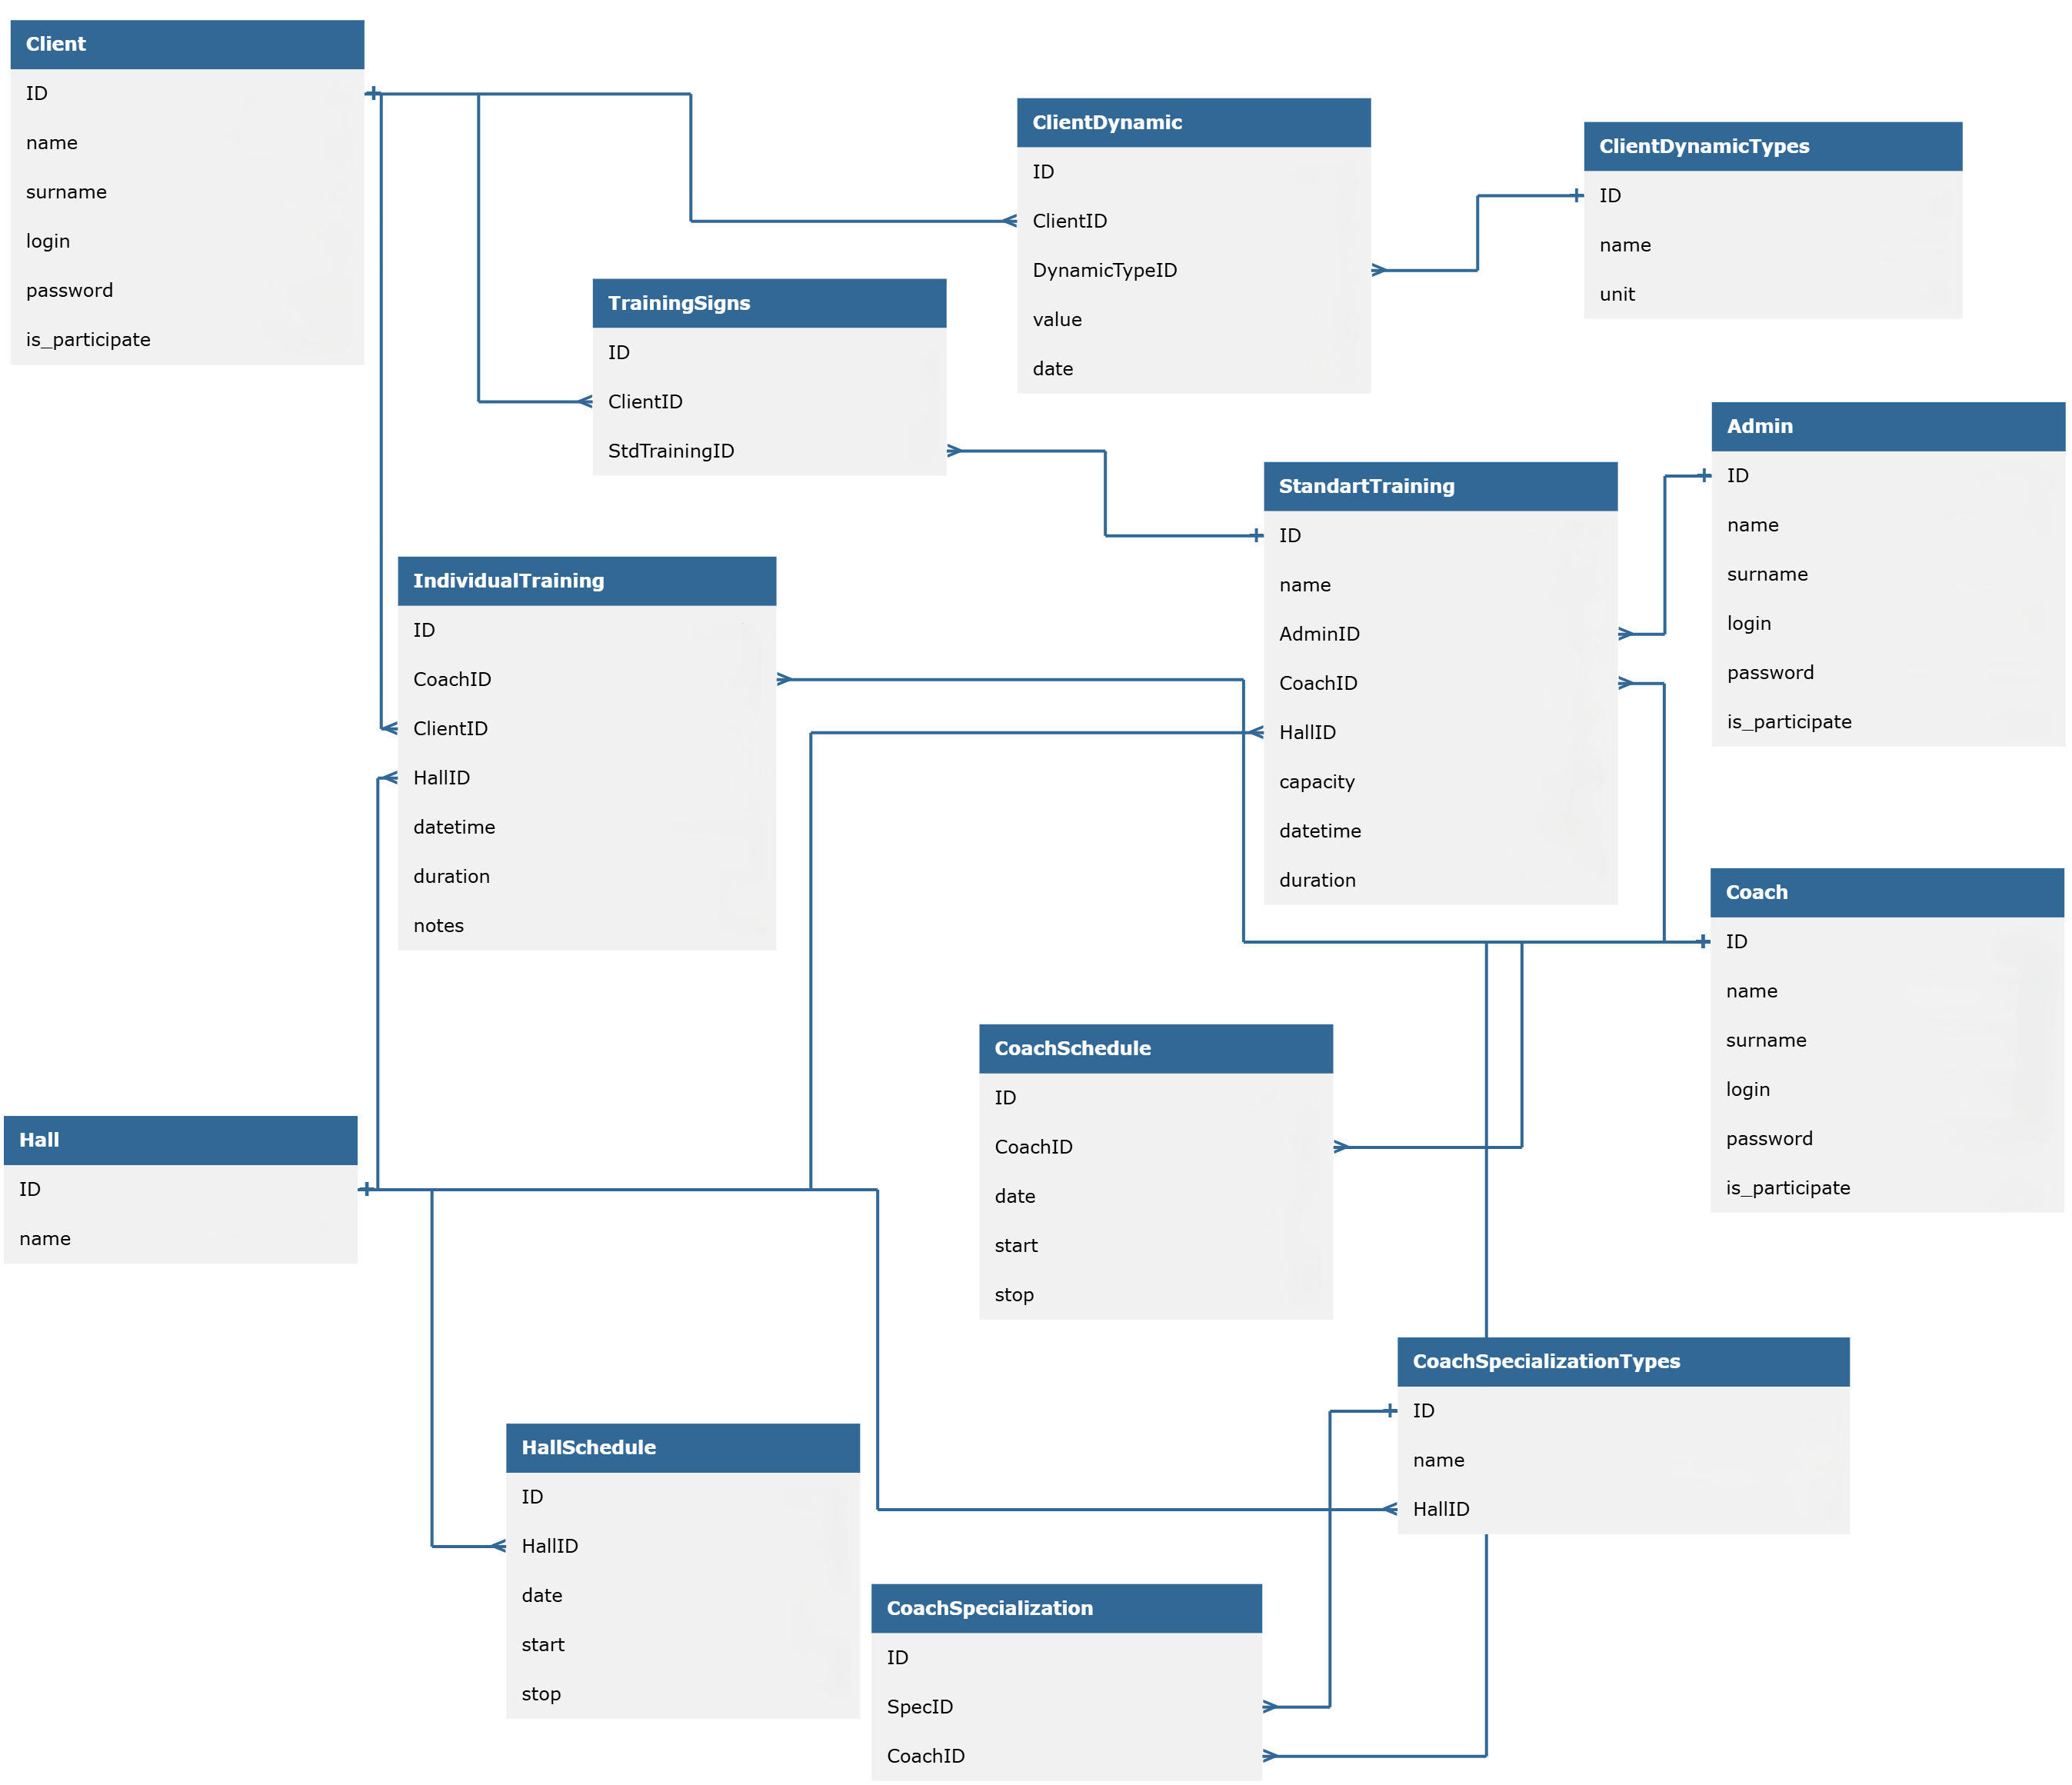
\includegraphics[height=0.65\textheight,angle=90]{img/database_diagram.png}
	\caption{Диаграмма проектируемой базы данных}
	\label{fig:database_diagram}
\end{figure}

\clearpage

\section{Описание проектируемых ограничений целостности базы данных}

\begin{enumerate}
    \item Таблица Coach (Тренер):
    \begin{itemize}
        \item[---] Поле name не может быть пустым;
        \item[---] Поле name должно содержать только буквы (латинские или кириллические);
        \item[---] Поле surname не может быть пустым;
        \item[---] Поле surname должно содержать только буквы (латинские или кириллические);
        \item[---] Поле login не может быть пустым;
        \item[---] Поле login должно содержать только латинские буквы и цифры;
        \item[---] Поле password не может быть пустым;
        \item[---] Пароль должен быть длиной не менее 8 символов;
        \item[---] Логин должен быть уникальным;
        \item[---] Длина логина должна быть от 8 до 10 символов;
        \item[---] Поле is\_participate по умолчанию должно быть истинным.
    \end{itemize}

    \item Таблица CoachSpecializationTypes (Типы специализаций тренеров):
    \begin{itemize}
        \item[---] Поле name не может быть пустым;
        \item[---] Поле HallID является внешним ключом, ссылающимся на таблицу Hall;
        \item[---] Поле name должно быть уникальным. 
    \end{itemize}

    \item Таблица CoachSpecialization (Специализации тренеров):
    \begin{itemize}
        \item[---] Поле SpecID является внешним ключом, ссылающимся на таблицу CoachSpecializationTypes;
        \item[---] Поле CoachID является внешним ключом, ссылающимся на таблицу Coach;
        \item[---] Пара SpecID, CoachID должна быть уникальной.
    \end{itemize}

    \item Таблица CoachSchedule (Расписание тренеров):
    \begin{itemize}
        \item[---] Поле CoachID является внешним ключом, ссылающимся на таблицу Coach;
        \item[---] Поле date не может быть пустым;
        \item[---] Поле start не может быть пустым;
        \item[---] Поле stop не может быть пустым;
        \item[---] Комбинация CoachID и date должна быть уникальной.
    \end{itemize}

    \item Таблица Client (Клиент):
    \begin{itemize}
        \item[---] Поле name не может быть пустым;
        \item[---] Поле name должно содержать только буквы (латинские или кириллические);
        \item[---] Поле surname не может быть пустым;
        \item[---] Поле surname должно содержать только буквы (латинские или кириллические);
        \item[---] Поле login не может быть пустым;
        \item[---] Поле login должно содержать только латинские буквы и цифры;
        \item[---] Поле password не может быть пустым;
        \item[---] Пароль должен быть длиной не менее 8 символов;
        \item[---] Логин должен быть уникальным;
        \item[---] Длина логина должна быть от 8 до 10 символов;
        \item[---] Поле is\_participate по умолчанию должно быть истинным.
    \end{itemize}

    \item Таблица ClientDynamicTypes (Типы динамических данных клиента):
    \begin{itemize}
        \item[---] Поле name не может быть пустым;
        \item[---] Поле unit не может быть пустым;
        \item[---] Поле name должно быть уникальным.
    \end{itemize}

    \item Таблица ClientDynamic (Динамические данные клиента):
    \begin{itemize}
        \item[---] Поле ClientID является внешним ключом, ссылающимся на таблицу Client;
        \item[---] Поле DynamicTypeID является внешним ключом, ссылающимся на таблицу ClientDynamicTypes;
        \item[---] Поле value не может быть пустым;
        \item[---] Поле date не может быть пустым;
        \item[---] Тройка ClientID, DynamicTypeID, date должна быть уникальной.
    \end{itemize}

    \item Таблица Admin (Администратор):
    \begin{itemize}
        \item[---] Поле name не может быть пустым;
        \item[---] Поле name должно содержать только буквы (латинские или кириллические);
        \item[---] Поле surname не может быть пустым;
        \item[---] Поле surname должно содержать только буквы (латинские или кириллические);
        \item[---] Поле login не может быть пустым;
        \item[---] Поле login должно содержать только латинские буквы и цифры;
        \item[---] Поле password не может быть пустым;
        \item[---] Пароль должен быть длиной не менее 8 символов;
        \item[---] Логин должен быть уникальным;
        \item[---] Длина логина должна быть от 8 до 10 символов;
        \item[---] Поле is\_participate по умолчанию должно быть истинным.
    \end{itemize}

    \item Таблица StandartTraining (Групповые мероприятия):
    \begin{itemize}
        \item[---] Поле name не может быть пустым;
        \item[---] Поле name должно содержать только буквы (латинские или кириллические), может состоять из нескольких слов;
        \item[---] Поле name не может состоять только из пробелов;
        \item[---] Поле AdminID является внешним ключом, ссылающимся на таблицу Admin;
        \item[---] Поле CoachID является внешним ключом, ссылающимся на таблицу Coach;
        \item[---] Поле HallID является внешним ключом, ссылающимся на таблицу Hall;
        \item[---] Поле capacity не может быть пустым;
        \item[---] Вместимость должна быть больше 0;
        \item[---] Поле datetime не может быть пустым;
        \item[---] Поле duration не может быть пустым;
        \item[---] Длительность должна быть больше 0.
    \end{itemize}

    \item Таблица Hall (Спортивное пространство):
    \begin{itemize}
        \item[---] Поле name не может быть пустым;
        \item[---] Поле name должно содержать буквы (латинские или кириллические), цифры и дефисы, может состоять из нескольких слов;
        \item[---] Поле name не может состоять только из пробелов;
        \item[---] Поле name должно быть уникальным.
    \end{itemize}

    \item Таблица HallSchedule (Расписание спортивного пространства):
    \begin{itemize}
        \item[---] Поле HallID является внешним ключом, ссылающимся на таблицу Hall;
        \item[---] Поле date не может быть пустым;
        \item[---] Поле start не может быть пустым;
        \item[---] Поле stop не может быть пустым;
        \item[---] Комбинация HallID и date должна быть уникальной.
    \end{itemize}

    \item Таблица TrainingSigns (Записи на тренировки):
    \begin{itemize}
        \item[---] Поле ClientID является внешним ключом, ссылающимся на таблицу Client;
        \item[---] Поле StdTrainingID является внешним ключом, ссылающимся на таблицу StandartTraining;
        \item[---] Пара ClientID, StdTrainingID должна быть уникальной.
    \end{itemize}

    \item Таблица IndividualTraining (Индивидуальные тренировки):
    \begin{itemize}
        \item[---] Поле CoachID является внешним ключом, ссылающимся на таблицу Coach;
        \item[---] Поле ClientID является внешним ключом, ссылающимся на таблицу Client;
        \item[---] Поле HallID является внешним ключом, ссылающимся на таблицу Hall;
        \item[---] Поле datetime не может быть пустым;
        \item[---] Поле duration не может быть пустым;
        \item[---] Длительность должна быть больше 0;
        \item[---] Пара CoachID, datetime должна быть уникальной.
    \end{itemize}
\end{enumerate}

\section{Описание проектируемых функций в формате схемы}

На рисунке \ref{fig:sheme_get_coach_specializations} представлена схема работы функции 
get\_coach\_specializ-

ations, которая получает список специализаций тренера.

\begin{figure}[H]
	\centering
	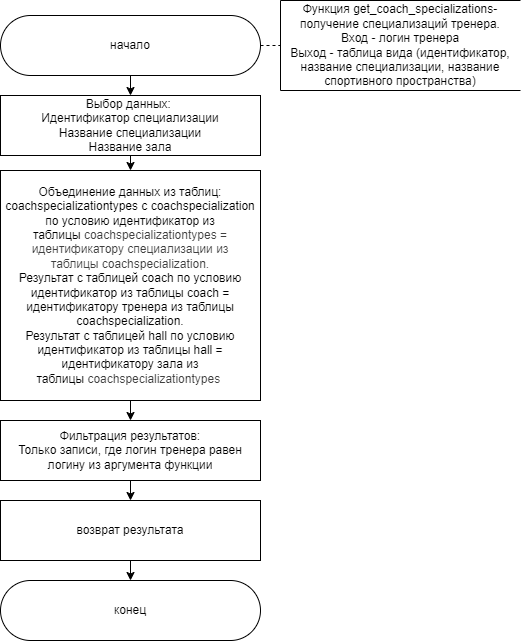
\includegraphics[height=0.7\textheight]{shemes/get_coach_specializations.drawio.png}
	\caption{Схема алгоритма функции get\_coach\_specializations}
	\label{fig:sheme_get_coach_specializations}
\end{figure}

На рисунке \ref{fig:show_available_events} представлена схема работы функции 
show\_available\_events, которая получает список доступных для записи мероприятий.

\begin{figure}[H]
	\centering
	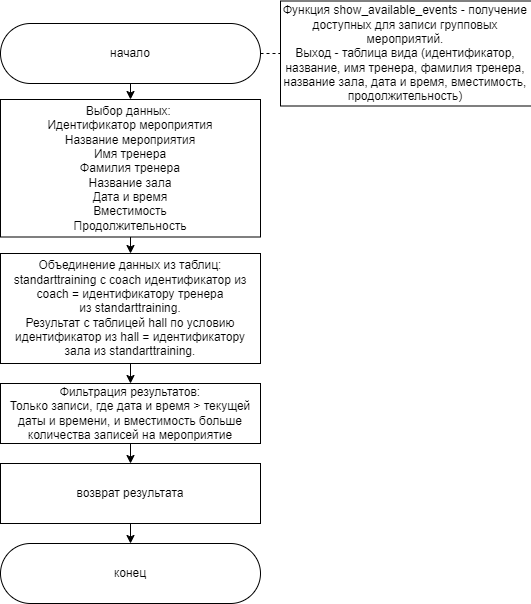
\includegraphics[height=0.7\textheight]{shemes/show_available_events.drawio.png}
	\caption{Схема алгоритма функции show\_available\_events}
	\label{fig:show_available_events}
\end{figure}

На рисунке \ref{fig:register_client_for_training} представлена схема работы функции 
register\_client\_for\_-

training, которая выполняет регистрацию клиента на мероприятие.

\begin{figure}[H]
	\centering
	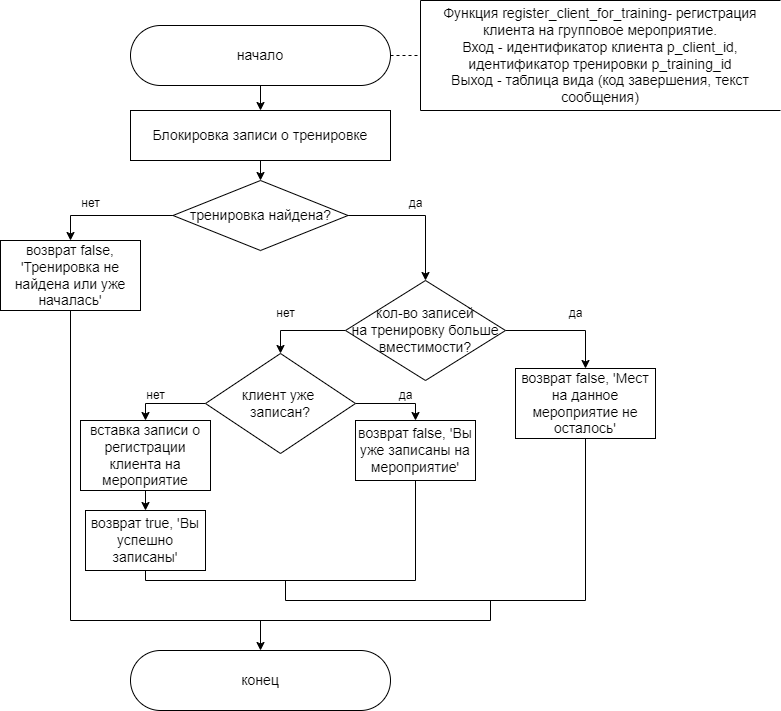
\includegraphics[height=0.58\textheight]{shemes/register_client_for_training.drawio.png}
	\caption{Схема алгоритма функции register\_client\_for\_training}
	\label{fig:register_client_for_training}
\end{figure}

\section{Описание проектируемой ролевой модели на уровне базы данных}

Ролевая модель состоит из трёх ролей: клиента, тренера и администратора.

\begin{enumerate}
    \item Администратор имеет следующие возможности:
    \begin{itemize}
        \item[---] Просмотр, добавление и удаление данных в таблице ClientDynamicTypes;
        \item[---] Просмотр данных в таблице Hall;
        \item[---] Просмотр данных в таблице IndividualTraining;
        \item[---] Просмотр, добавление и изменение данных в таблице CoachSchedule;
        \item[---] Просмотр данных в таблице CoachSpecializationTypes;
        \item[---] Просмотр, добавление и удаление данных в таблице CoachSpecialization;
        \item[---] Просмотр, добавление и изменение данных в таблице HallSchedule;
        \item[---] Просмотр, добавление и изменение данных в таблице Client;
        \item[---] Просмотр, добавление и изменение данных в таблице Coach;
        \item[---] Просмотр, добавление и изменение данных в таблице Admin;
        \item[---] Полный доступ (просмотр, удаление, добавление, изменение) к таблице StandartTraining.
    \end{itemize}

    \item Клиент имеет следующие возможности:
    \begin{itemize}
        \item[---] Просмотр данных в таблице ClientDynamicTypes;
        \item[---] Просмотр, добавление и удаление данных в таблице ClientDynamic;
        \item[---] Просмотр и изменение данных в таблице StandartTraining;
        \item[---] Просмотр данных в таблице Hall;
        \item[---] Просмотр данных в таблице Coach;
        \item[---] Просмотр и удаление данных в таблице IndividualTraining;
        \item[---] Просмотр, добавление и удаление данных в таблице TrainingSigns.
    \end{itemize}

    \item Тренер имеет следующие возможности:
    \begin{itemize}
        \item[---] Просмотр, изменение и добавление данных в таблицу CoachSchedule;
        \item[---] Просмотр данных в таблице StandartTraining;
        \item[---] Просмотр данных в таблице Admin;
        \item[---] Просмотр данных в таблице Coach;
        \item[---] Просмотр даных в таблице Hall;
        \item[---] Полный доступ (просмотр, удаление, добавление, изменение) к таблице IndividualTraining;
        \item[---] Просмотр данных в таблице Client;
        \item[---] Просмотр данных в таблице CoachSpecializationTypes;
        \item[---] Просмотр данных в таблице CoachSpecialization.
    \end{itemize}
\end{enumerate}